\section{Database View}

In this section is described the design of the database that will be used for the \textit{TrackMe} system. 

\begin{figure}[H]
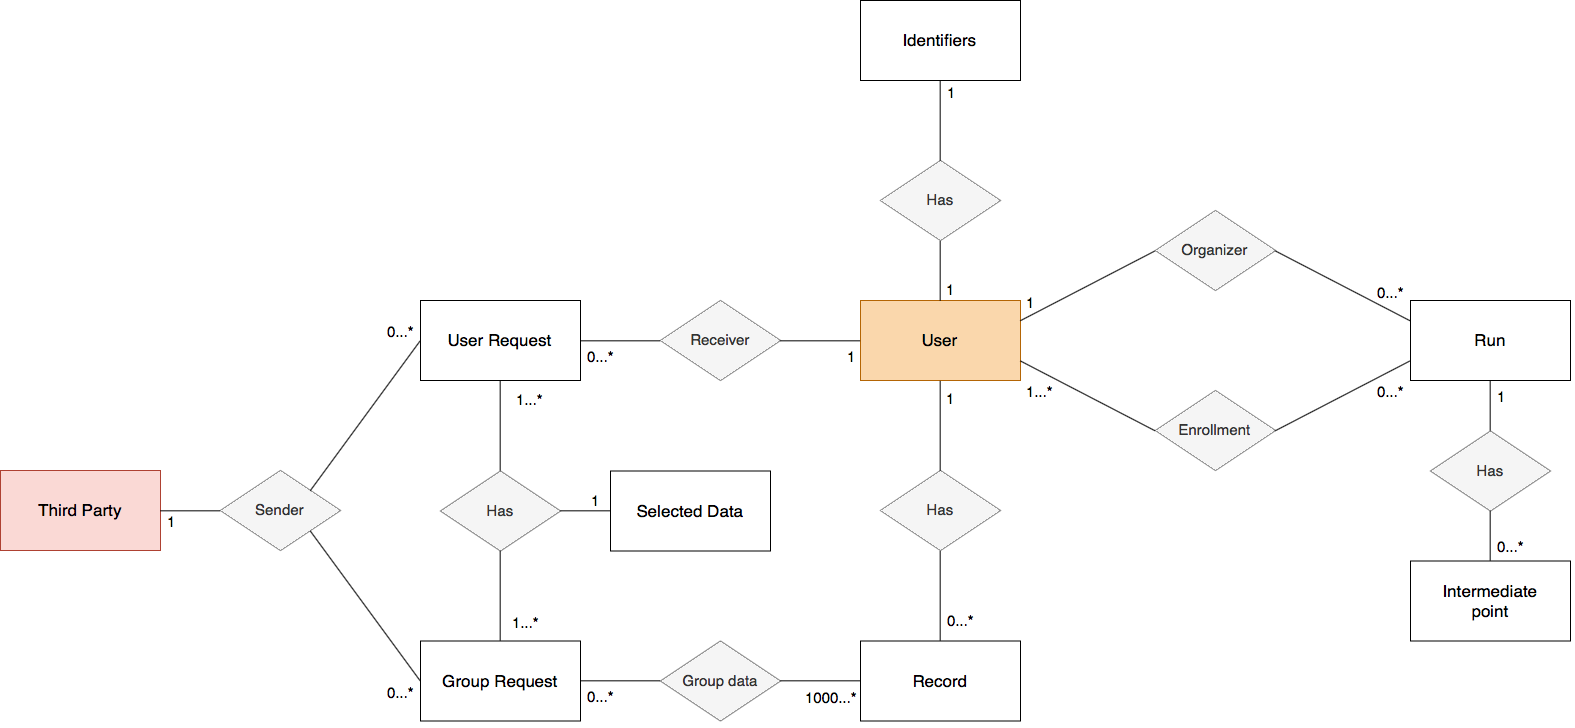
\includegraphics[scale=0.27,keepaspectratio]{DD/Pictures/ER-diagram.png}
\centering
\caption{Simplified ER diagram for the \textit{TrackMe} system}
\end{figure}

The picture above shows the main entities of the database. There is a \textit{User} entity, used to store the personal information of individual users that is requested at sign up. Every user has many records associated to itself, each of them containing location and health data. This information is put in the \textit{Record} entity. The \textit{Third Party} entity contains meaningful data about the company that signed up to the \textit{TrackMe} system. Third parties can make requests to the system in order to get access to user data, so the \textit{Third Party} entity is related with the \textit{User Request} and the \textit{Group Request} entities. Both these entities contain information about the request, such as its status and the specific type of data to be accessed, but there is an important difference between the two regarding the anonymity of data. While a user request is sent to an individual user directly, a group request has a higher scope, and the data that 
is accessed after this type of request must be completely anonymous. The sender of the request must not get access to the personal data of the users that have generated the records. To enforce this, the \textit{Group Request} entity is not related with \textit{User}, but instead directly with \textit{Record}. This solution is permitted by the use of anonymous identifiers, present in the \textit{Record} entity, that have a 1 to 1 relation with the users of the system.

The \textit{Track4Run} service is represented by the Run entity, which has the information about the location, time and participants.

The \textit{AutomatedSOS} service does not rely on a complex data structure so it’s not displayed in the simplified ER diagram. Nevertheless, two attributes are present in the \textit{User} and \textit{Record} entities: the \textit{SosEnabled} attribute is a flag that indicates if the service is enabled or not; the \textit{isEmergency} attribute indicates if the record contains critical health parameters.

\begin{figure}[H]
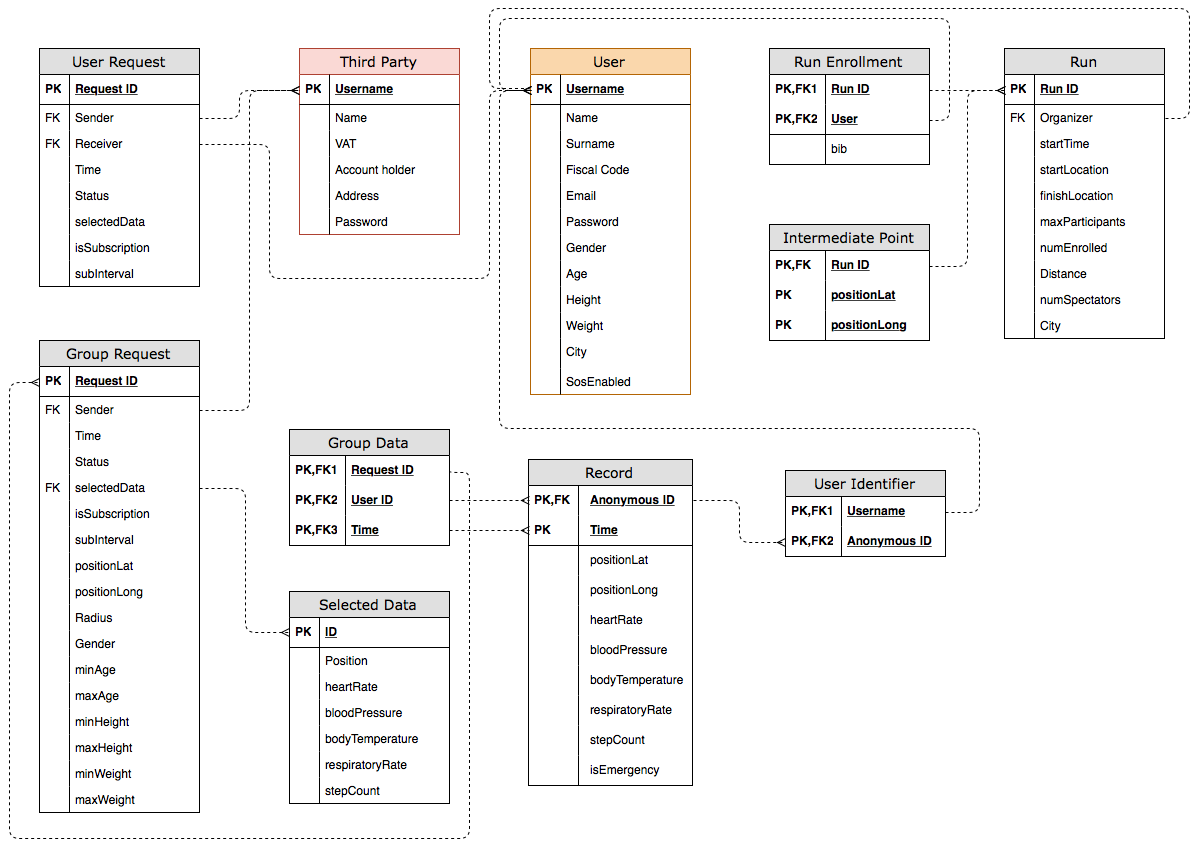
\includegraphics[scale=0.34,keepaspectratio]{DD/Pictures/ER-tables.png}
\centering
\caption{Tables and relative attributes of the \textit{TrackMe} database}
\end{figure}